\documentclass[12pt]{article}

\usepackage[a4paper, margin=1in]{geometry}
\usepackage{graphicx}
\usepackage[absolute, overlay]{textpos}
\usepackage{fancyhdr}
\usepackage{siunitx}
\usepackage{tikz}
\usepackage{pgfplots}
\usetikzlibrary{decorations.pathmorphing}
\usetikzlibrary{math}
\usetikzlibrary{calc}

\pgfplotsset{compat=1.18}

\pagestyle{fancy} %for footers

\newcommand{\customsubject}{}   
\newcommand{\customtitle}{}

\newcounter{questionpartcounter}                  %Setup for question part counter for a,b,c listing
\renewcommand{\thequestionpartcounter}
{\alph{questionpartcounter}}

\newcounter{questionpartpartcounter}                  %Setup for question part  partcounter for a,b,c listing
\renewcommand{\thequestionpartpartcounter}
{\roman{questionpartcounter}}

\pagestyle{fancy} %for footers
\renewcommand{\headrulewidth}{0pt}
\fancyhf{}
\fancyfoot[R]{\thepage}

\newenvironment{worksheet}[2]
{
    
    \global\renewcommand{\customtitle}{#1}
    \global\renewcommand{\customsubject}{#2}


    \begin{textblock*}{5cm}(0.4cm,0.4cm)
   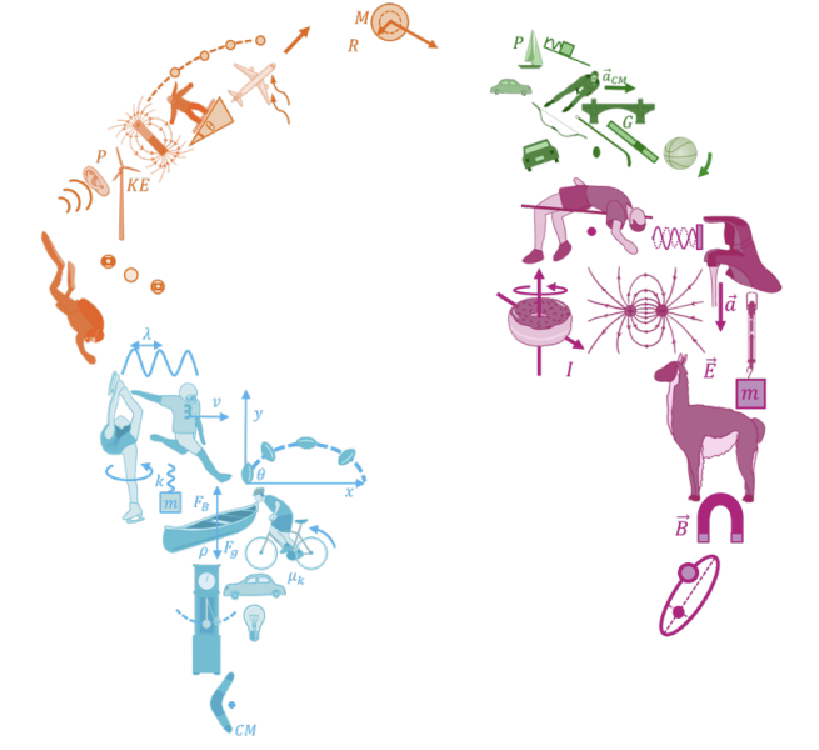
\includegraphics[width=4cm]{include/figures/bmdwlogo}
\end{textblock*}

    \vspace*{-1cm}
    
    {\large\textbf{\begin{center}\customtitle\end{center}}}

    \begin{center}\customsubject\end{center}
    
    \vspace{0.3cm}
    
    \hspace*{-1.5cm}\textbf{Name:\ \rule{4cm}{0.4pt}}\; 
    \textbf{Student \#: \ \rule{3cm}{0.4pt}}\;
    \textbf{Student Email \#: \ \rule{1.53cm}{0.4pt}}

    \vspace{0.5cm}

    
    \begin{enumerate}
}
{
    \end{enumerate}
   % \begin{textblock*}{10cm}(1cm, 28cm) {\footnotesize \scriptsize \customsubject}
    
%\end{textblock*}
}



\newcommand{\question}[2][1cm]{%
    \item
    \setcounter{questionpartcounter}{0}
    \setcounter{questionpartpartcounter}{0}
    {#2}
    \vspace{#1}
}

\newcommand{\questionpart}[2][1cm]{%
    \setcounter{questionpartpartcounter}{0}
    \stepcounter{questionpartcounter}
    (\thequestionpartcounter)~#2
    \vspace{#1}
}

\newcommand{\questionpartpart}[2][1cm]{%
      \stepcounter{questionpartpartcounter}
      \thequestionpartpartcounter.~#2
      \vspace{#1}
}

\newcommand{\operation}[1]{%
{\large $
#1
$}
}




\begin{document}

\begin{worksheet}{Phys 101 Worksheet}{Comparing Model and Experiment}

\question[0.1cm]{Suppose there's a theory "Dogs cannot be born with naturally blue fur."Can this theory be proven to be true? \textbf{Explain} why or why not.}

This theory \textbf{cannot be proven to be true}. It can only be disproved once a dog with naturally blue fir is discovered.

\vspace{2cm}

\question[0cm]{Suppose you're a butterfly researcher. You find that rarer butterflies appear to be faster, and flutter their wings at a higher rate than more common butterflies. You invent a new unit, a "Whimsy" (denoted as $W$), which is the \textbf{product} the maximum velocity of a given species of butterfly, $v$,  and the frequency at which it flaps its wings $f$.}

\questionpart[0cm]{Explicitly write out the formula to calculate Whimsiness. What are it's dimensions?}

\textbf{$W = vf$. It has dimenions of: $\frac{L}{T^2}$}

\vspace{1.5cm}

\questionpart[0cm]{ Suppose now you want to create a formula that could predict the most whimsical butterfly any given butterfly catching machine could catch knowing only its mass, $m$ and the maximum force it can swing with $F_s$. Write a possible solution (within a constant) that could be a solution to the problem.}

$W = k\frac{F_s}{m}$

\vspace{2.5cm}

\questionpart[0cm]{Does the formula you've devised make sense? Explain wy or why not}

It makes sense because the formula is dimensionally sound. As well, a bigger machine would be harder to carry and thus would not be able to catch as whimsical butterflies which will be faster and thus more difficult to catch.

\end{worksheet}


\end{document}